%%%%%%%%%%%%%%%%%%%%%%%%%%%%%%%%%%%%%%%%%
% The Legrand Orange Book
% LaTeX Template
% Version 2.1.1 (14/2/16)
%
% This template has been downloaded from:
% http://www.LaTeXTemplates.com
%
% Original author:
% Mathias Legrand (legrand.mathias@gmail.com) with modifications by:
% Vel (vel@latextemplates.com)
%
% License:
% CC BY-NC-SA 3.0 (http://creativecommons.org/licenses/by-nc-sa/3.0/)
%
% Compiling this template:
% This template uses biber for its bibliography and makeindex for its index.
% When you first open the template, compile it from the command line with the 
% commands below to make sure your LaTeX distribution is configured correctly:
%
% 1) pdflatex main
% 2) makeindex main.idx -s StyleInd.ist
% 3) biber main
% 4) pdflatex main x 2
%
% After this, when you wish to update the bibliography/index use the appropriate
% command above and make sure to compile with pdflatex several times 
% afterwards to propagate your changes to the document.
%
% This template also uses a number of packages which may need to be
% updated to the newest versions for the template to compile. It is strongly
% recommended you update your LaTeX distribution if you have any
% compilation errors.
%
% Important note:
% Chapter heading images should have a 2:1 width:height ratio,
% e.g. 920px width and 460px height.
%
%%%%%%%%%%%%%%%%%%%%%%%%%%%%%%%%%%%%%%%%%

%----------------------------------------------------------------------------------------
%	PACKAGES AND OTHER DOCUMENT CONFIGURATIONS
%----------------------------------------------------------------------------------------

\documentclass[11pt,fleqn]{book} % Default font size and left-justified equations

\usepackage{ifthen} 
\newboolean{VersionProf}
\setboolean{VersionProf}{false}

\usepackage{wasysym}
\usepackage{esint} % various fancy integral symbols
\usepackage{tikz}
\usepackage{tikz-3dplot}
\usepackage{pgfplots}
\pgfplotsset{compat=1.17}
\usetikzlibrary{patterns}
\usepackage{tkz-euclide} 
\usepackage{mathtools}
\usepackage{xurl}
\usepackage[version=4,arrows=pgf-filled,
textfontname=sffamily,
mathfontname=mathsf]{mhchem}
\usepackage{gensymb}
\usepackage{tabularray}
\usepackage{csquotes}

\usepackage[french]{babel}
\usepackage{dingbat}

\usepackage{environ}
\usepackage{wrapfig}

\NewEnviron{solution}{%
    \ifthenelse{\boolean{VersionProf}}{\begin{solutionA}
        \BODY%*
        \end{solutionA}
    }{%
        \relax%
    }%
}%

\usetikzlibrary {arrows.meta} 

\newcommand{\degC}{{\degree}C}
\newcommand{\dd}{\mathrm{d}}
\newcommand{\div}{\mathrm{div}}
\newcommand{\rot}{\vv{\mathrm{div}}}
\newcommand{\grad}{\vv{\mathrm{grad}}}

\tikzset{
    support/.style={
        pattern=north east lines,
        draw=none,
        minimum width=0.3,
        minimum height=0.6
    }
    ,>=latex
}

\usepackage[d]{esvect}

%SPECIFIC TO THIS CHAPTER
\usepackage{physics}
\usepackage{ifthen}
\usepackage[outline]{contour} % glow around text
\usetikzlibrary{calc} % for pic
\usetikzlibrary{angles,quotes} % for pic
\usetikzlibrary{patterns}
\tikzset{>=latex} % for LaTeX arrow head
\contourlength{1.2pt}

\colorlet{myred}{red!65!black}
\definecolor{myred}{RGB}{127,0,255}
\tikzstyle{ground}=[preaction={fill,top color=black!10,bottom color=black!5,shading angle=20},
                    fill,pattern=north east lines,draw=none,minimum width=0.3,minimum height=0.6]
\tikzstyle{mass}=[line width=0.6,myred,fill=myred!40,rounded corners=1,
                  top color=myred!40,bottom color=myred!20,shading angle=20]
\tikzstyle{rope}=[myred!30,line width=1.2,line cap=round] %very thick

% FORCES SWITCH
\tikzstyle{force}=[->,myred,ultra thick,line cap=round]
\tikzstyle{Fproj}=[force,myred!60]
\newboolean{showforces}
\setboolean{showforces}{true}
%----------------------------------------------------------------------------------------

\input{structure} % Insert the commands.tex file which contains the majority of the structure behind the template

\begin{document}

%----------------------------------------------------------------------------------------
%	TABLE OF CONTENTS
%----------------------------------------------------------------------------------------

%\usechapterimagefalse % If you don't want to include a chapter image, use this to toggle images off - it can be enabled later with \usechapterimagetrue

\chapterimage{filmB.jpg} % Table of contents heading image

%\pagestyle{empty} % No headers

%\tableofcontents % Print the table of contents itself

%\cleardoublepage % Forces the first chapter to start on an odd page so it's on the right

%\pagestyle{fancy} % Print headers again



%\part{\'{E}lectromagnétisme}

\setcounter{chapter}{8}

\chapter{Interférences par division de front d'onde}

\section{Les trous d'Young}

Dans le chapitre précédent, nous avons étudié la possibilité d'avoir des interférences par division d'amplitude, ce que l'on réalisait typiquement avec un dioptre optique ou une lame semi-réfléchissante. Nous allons ici nous intéresser à un autre type d'interférences, qui correspondent à l'une des perières expériences menées ppar Thomas Young : les interférences par division de front d'onde.

\begin{definition}
	On dit que l'on a des interférences par division de front d'onde lorsque les deux rayons qui interfèrent sont issus de deux rayons distincts qui émergent de la source.
\end{definition}

\subsection{Observations expérimentales}

L'espérience des trous d'Young peut être rélisée à partir d'une source ponctuelle monochromatique (en général, un laser ou une fente source), avec laquelle on éclaire une plaque percée de deux trous. On observe alors des franges superposées à une figure de diffraction, comme cela est visible sur la figure suivante :
\begin{figure}[htbp]
	\centering 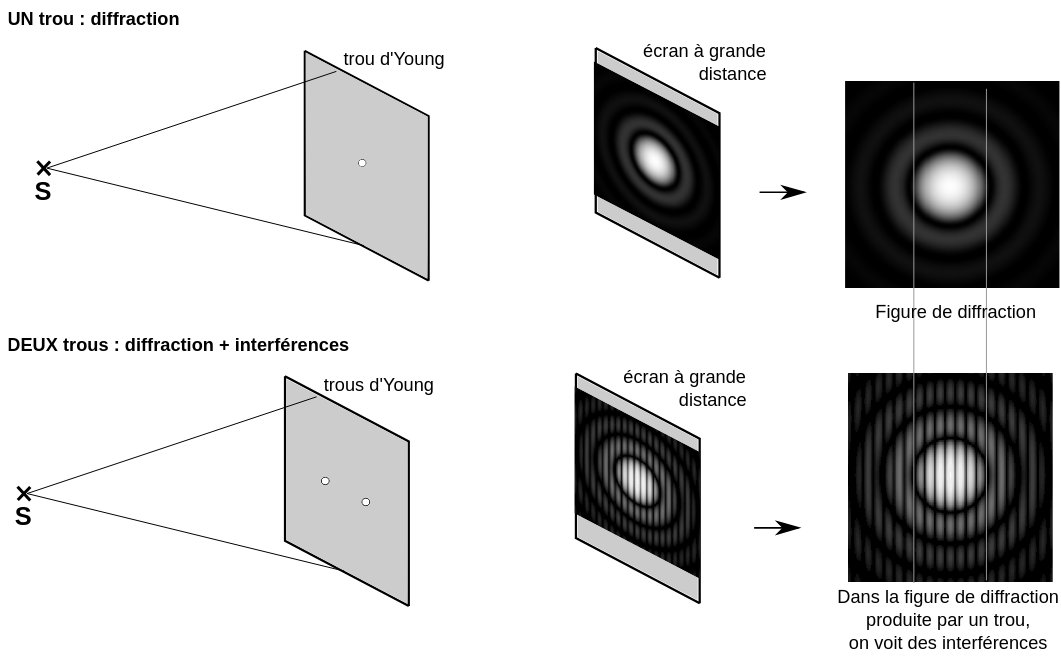
\includegraphics[width=\linewidth]{trous_young_observations.png}
	\caption{Observations réalisées à l'aide de l'expérience des trous d'Young. On constate un phénomène d'interférences, mais également un phénomène de diffraction. Source de cette figure et quasiment toutes les suivantes : ploy de cours de Etienne Thibierge.}
\end{figure}

On observe alors deux phénomènes :

\subsubsection{Diffraction}
Le premier phénomène est un phénomène de diffraction, qui se produit également lorsue l'on n'a qu'un seul trou. En effet, le trou diffracte la lumùière dans un cône qui est d'autant plus large que le trou a un diamètre petit devant la longueur d'onde de l'onde considérée. On rappelle la propriété suivante :

\begin{figure}[htbp]
	\centering 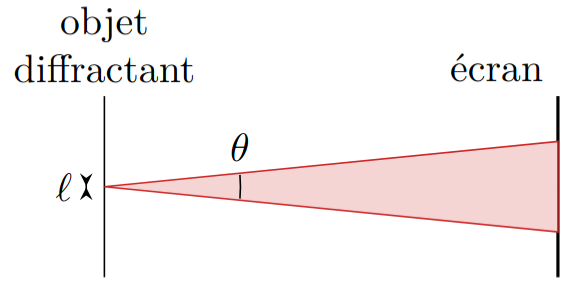
\includegraphics[width=0.3\linewidth]{diffraction.png}
	\caption{Phénomène de diffraction.}
\end{figure}

\begin{proposition}[Diffraction par un trou]
	La diffraction de la lumière par un objet de taille $\ell$ dévie les rayons dans un cône de largeur angulaire :
	\begin{equation}
		\theta \sim \frac{\lambda}{\ell}
	\end{equation}
	où $\lambda$ est la longueur d'onde de l'onde lumineuse considérée.
	Pour un trou, la figure a l'allure d'un cercle central entouré d'anneaux brillants successifs.
\end{proposition}

\subsubsection{Interférences}
Les interférences n'apparaissent que lorsque l'on a au moins deux trous. Ceci est dû à la présence de deux rayons lumineux qui vont interférer en tout point de l'espace :
\begin{itemize}
	\item Le rayon issu de $S$, qui passe par le trou $S_1$, et est diffracté par ce trou vers le point $M$.
	\item Le rayon issu de $S$, qui passe par le trou $S_2$, et est diffracté par ce trou vers le point $M$.
\end{itemize}
Ces deux rayons peuvent interférer si et seulement si $M$ se trouve dans les cônes de diffraction des deux trous, c'est ce que l'on va nommer le champ d'interférences :
\begin{definition}
	On appelle champ d’interférences la zone de l’espace dans laquelle les ondes diffractées par chacun des deux trous se superposent.
\end{definition}
Dans le champ d'interférences, on va observer des interférences dues à la différence de marche entre les trajets de chacun des rayons lumineux. Ceci se comprend intuitivement par le schéma historique de Thomas Young, dont une version moderne est présentée ici :

\begin{figure}[htbp]
	\centering 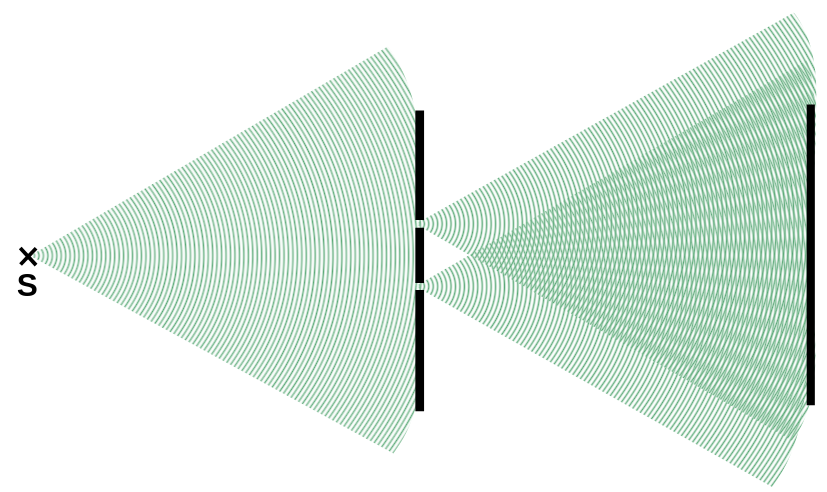
\includegraphics[width=0.7\linewidth]{champ_interferences.png}
	\caption{Schéma des fronts d'onde dans l'expérience des trous d'Young. La largeur angulaire des deux cônes de droite correspond à l'angle $\theta$ de diffraction du schéma précédent, et le champ d'interférences est la superposition de ces deux cônes.}
\end{figure}

En tout point $M$ du champ d'interférences, il existe deux et seulement deux rayons issus de la source primaire $S$ qui atteignent le point $M$. On en déduit que les interférences se produisent en tout point de l'espace, sans brouillage lié à la position du point $M$. Ainsi :
\begin{proposition}[Localisation des interférences]
	Les interférences par division de front d'onde ne sont jamais localisées : elles sont visibles en tout point de l'espace.
\end{proposition}

En pratique, bien que l'on constate que le phénomène de diffraction soit essentiel pour permettre les interférences, nous ne nous attacherons pas à sa description dans la suite de ce cours. Nous allons nous concentrer sur les interférences, et l'apparition des franges brillantes et sombres sur l'écran.

\subsection{Figure d'interférences}

\subsubsection{Interférences à grande distance}

Nous allons d'abord nous intéresser au cas d'interférences qui se produisent sur un écran situé à une distance $D$, grande mais finie, de la source lumineuse. Il s'agit d'un rappel de MPSI.

\begin{figure}[htbp]
	\centering 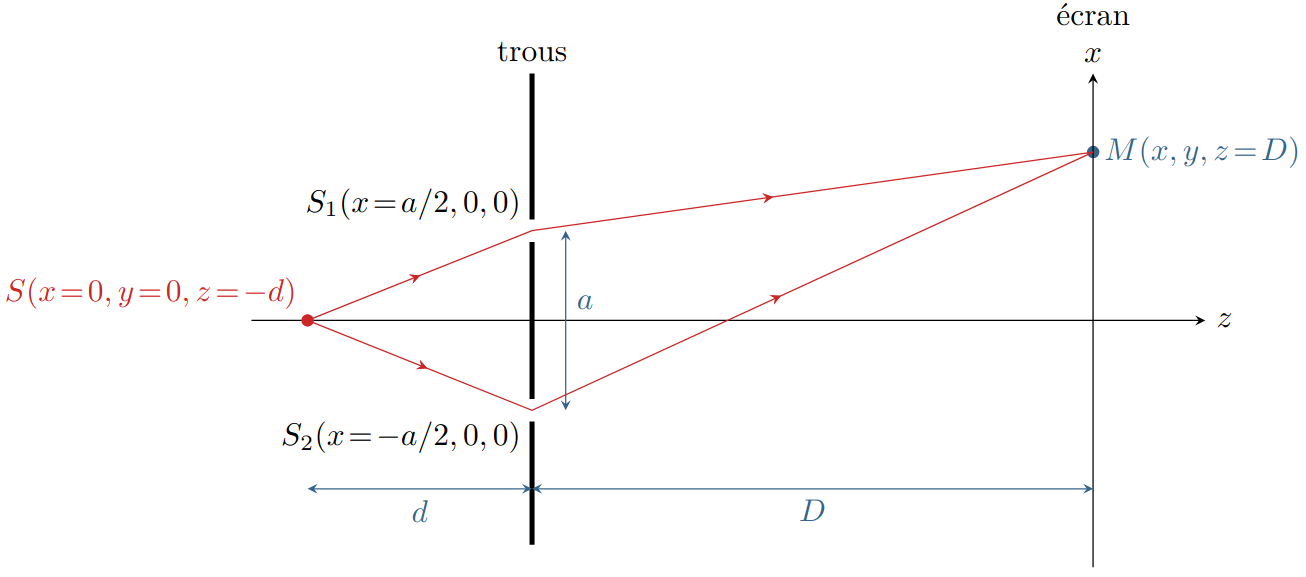
\includegraphics[width=\linewidth]{young_sans_lentille.png}
	\caption{Schéma de l'expérience des trous d'Young, où l'on observe les interférences à une distance finie $D$ des trous.}
\end{figure}

\begin{capex}
	Monter que la différence de marche s'écrit :
	\begin{equation}
		\delta = \frac{a x}{D}
	\end{equation}
\end{capex}


\subsubsection{Interférences à l'infini}

Il est également possible d'observer les interférences produites à l'infini de la même manière qu'avec l'interféromètre de Michelson : on regarde la figure d'interférences en plaçant l'écran dans le plan focal image d'une lentille située après les fentes.


\begin{figure}[htbp]
	\centering 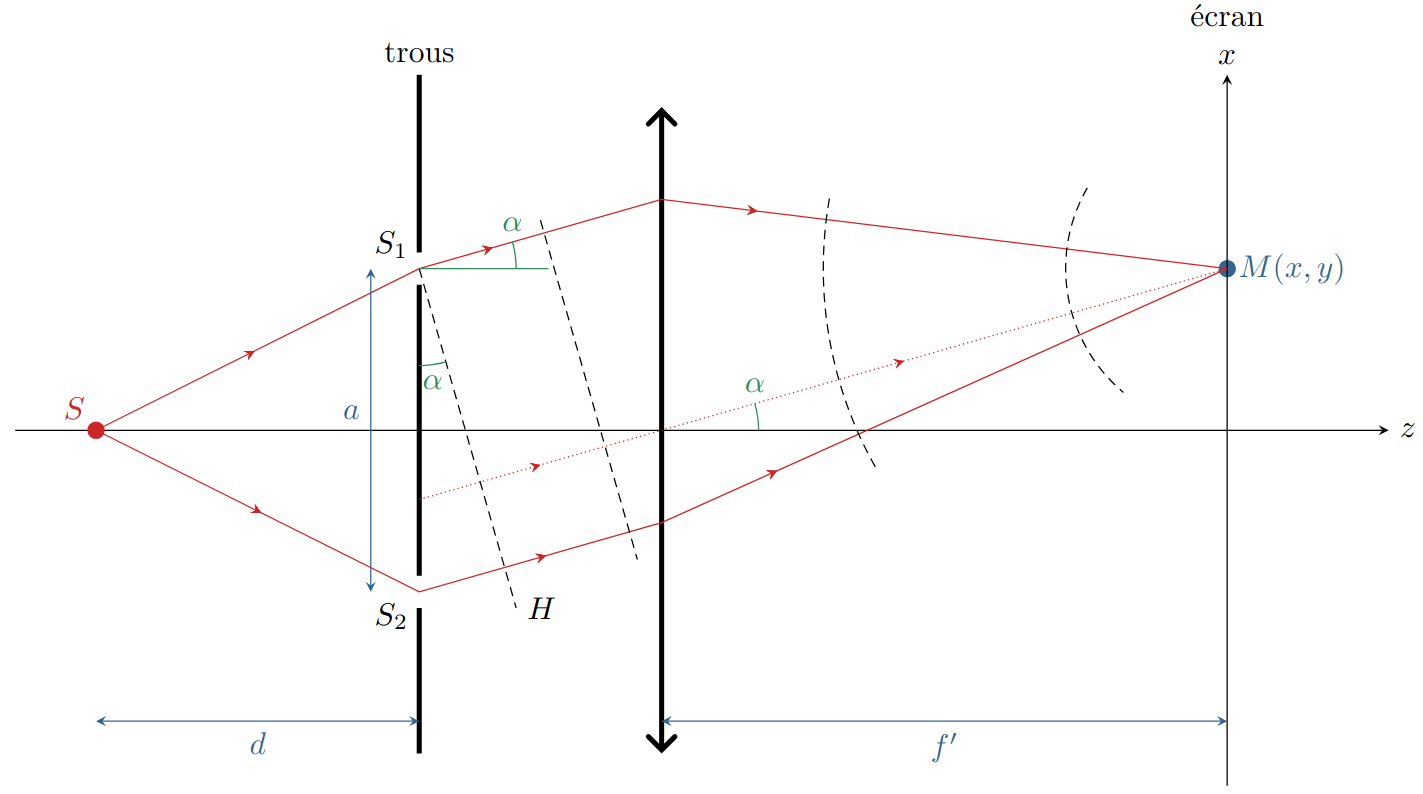
\includegraphics[width=\linewidth]{young_avec_lentille.png}
	\caption{Schéma de l'expérience des trous d'Young, où l'on observe les interférences à l'infini à l'aide d'une lentille. Les lignes en pointillés représentent des surfaces d'onde inverses, c'est-à-dire les surfaces d'onde qui correspondraient à une onde lumineuse émise en $M$. Ce ne sont pas des vraies surfaces d'onde (sinon il n'y aurait pas d'interférences en $M$).}
\end{figure}

\begin{capex}
	Monter que la différence de marche s'écrit :
	\begin{equation}
		\delta = \frac{a x}{f'}
	\end{equation}
\end{capex}

Dans la démonstration, on s'aidera notamment des propriétés sur les fronts d'onde vues au chapitre sur le modèle scalaire des ondes, et du principe de retour inverse de la lumière, qui se traduit en terme de chemin optique :
\begin{theorem}[Principe de retour inverse de la lumière]
	Si la lumière allait du point d’observation vers la source, alors les rayons lumineux seraient les mêmes.
	Il y a donc égalité des chemins optiques entre deux points $A$ et $B$ quel que soit le sens de parcours :
	\begin{equation}
		(AB) = (BA)
	\end{equation}
\end{theorem}
\begin{demonstration}
	La première phrase est un postulat vu en MPSI. La seconde se démontre simplement par la définition du chemin optique : les rayons direct et inverse étant identiques, ils parcourent la même distance dans des milieux de même indice optique $n$.
\end{demonstration}

\subsubsection{Interfrange et ordre d'interférences}

A partir de l'expression de la différence de marche, on peut retrouver l'allure de la figure d'interférences : il s'agit de franges verticales, d'égale épaisseur (analogue à la configuration du Michelson en coin d'air). Cette configuration aurait aussi pu être retrouvée par une analyse similaire à celle faite à la fin du chapitre 8, en remarquant que l'on a deux sources secondaires ponctuelles qui émettent en phase. 

Pour caractériser la figure, on définit l'interfrange :
\begin{definition}[Interfrange]
	On appelle interfrange la distance qui sépare le centre de deux franges brillantes (ou sombres) successives. On a alors :
	\begin{align}
		\varphi(x + i) &= \varphi(x) + 2 \pi  \\
		p(x+i) &= p(x) + 1 \\
		\delta(x+i) = \delta(x) + \lambda
	\end{align}
\end{definition}

\begin{capex}
	Exprimer l'interfrange $i$ en fonction de $a, \lambda$ et $D$ ou $f'$ (selon la configuration), puis exprimer l'ordre d'interférence $p$ en fonction de $i$ et $x$.
\end{capex}

\section{Cohérence et perte de contraste}

\subsection{Cohérence temporelle}

De la même manière qu'avec l'interféromètre de Michelson, la source n'est pas forcément constituée d'une unique fréquence. Elle a un temps de cohérence $\tau_c$ qui peut provoquer un brouillage des interférences. Ce temps de cohérence se traduit également par une longueur de cohérence, $\ell_c = c \tau_c$, représentant la longueur d'un train d'onde émis par la source.

\subsubsection{Source polychromatique}

On modélise une source émettant à différentes longueurs d'ondes de la manière suivante :

\begin{proposition}
	Une source non monochromatique peut être modélisée comme une collection de sources monochromatiques incohérentes, l'intensité totale étant la somme des intensités issues de chaque source.
\end{proposition}

\begin{capex}
	Déterminer la variation de l'ordre d'interférence, $\Delta p$, provoquée en un point $M$ de l'écran par une variation de longueur d'onde $\Delta \lambda$ de la source.
\end{capex}

On utilisera alors un critère de brouillage basé sur l'ordre d'interférence. En effet, lorsque l'on superpose des franges avec un écart d'ordre $\Delta p \neq 0$, les franges vont avoir tendance à se brouiller. Ce brouillage est total pour $\Delta p = 1$, et inexistant pour $\Delta p = 0$. On choisira donc $\Delta p = 0$, de manière arbitraire, comme critère de brouillage :
\begin{proposition}[Critère de brouillage]
	On peut considérer qu'il y a brouillage des interférences lorsque deux figures d'interférences se superposent avec un décalage de l'ordre d'interférence $\Delta p \ge \frac{1}{2}$. 
\end{proposition}
\begin{remark}
	Ce critère a ses limites, en effet, il ne prend pas en compte le fait que pour des décalages d'ordre entiers et supérieurs à $\frac{1}{2}$, les interférences peuvent se superposer sans se brouiller. Par exemple, ce critère ne permet pas d'expliquer des phénomènes tels que des figures d'interférences en "battements" pour les doublets comme nous l'avons vu avec l'interféromètre de Michelson. Le critère de brouillage est cependant utile pour les trous d'Young, qui ne permettent de toute façon de voir qu'un nombre limité de franges d'interférences.
\end{remark}


\begin{figure}[htbp]
	\centering 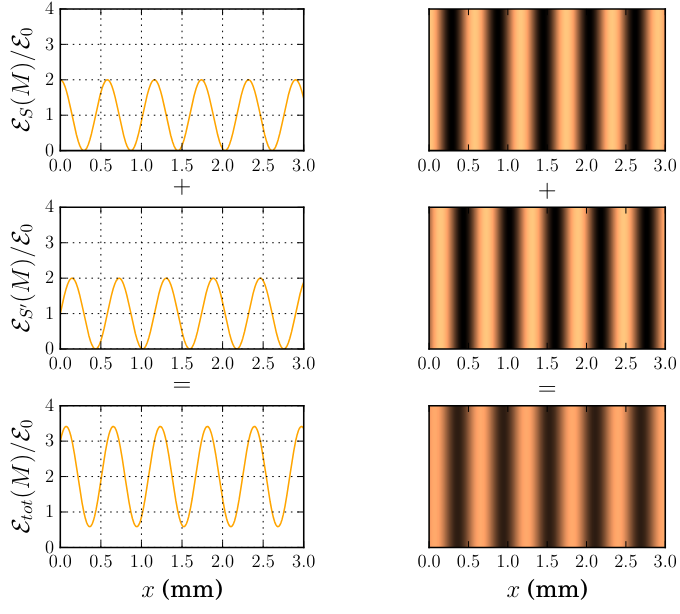
\includegraphics[width=0.5\linewidth]{brouillage.png}
	\caption{Superposition de deux figures d'interférences avec un décalage d'ordre d'environ 0.2.}
\end{figure}


Considérons alors une source qui a une longueur d'onde moyenne $\lambda_0$ et une largeur spectrale $\Delta \lambda_0$. Elle peut se modéliser par une infinité de sources dont les longueurs d'onde sont comprises entre $\lambda_0-\frac{\Delta \lambda_0}{2}$ et $\lambda_0+\frac{\Delta \lambda_0}{2}$. L'écart maximal entre $\lambda$ et la longueur d'onde moyenne est alors $\Delta \lambda = \frac{\Detla \lambda_0}{2}$.

On en déduit alors directement qu'il y a brouillage des interférences si :
\begin{equation}
	\Delta p \ge \frac{1}{2} \Leftrightarrow x \ge \frac{\lambda_0^2 D}{2 a \Delta \lambda_0}
\end{equation}
En d'autres termes :
\begin{proposition}
	Dans le dispositif des fentes d'Young, un élargissement spectral de la source produit un brouillage des interférences au-delà d'une distance maximale :
	\begin{equation}
		x_{max} = \frac{\lambda_0^2 D}{a \Delta \lambda_0}
	\end{equation}
	où $\lambda_0$ et $\Delta \lambda_0$ sont la longueur d'onde moyenne et la largeur spectrale de la source.
\end{proposition}

\subsubsection{Interprétation avec le modèle des trains d'onde}

On peut également utiliser le modèle des trains d'ondes : pour que deux ondes puissent interférer, la différence de marche doit être inférieure à la longueur de cohérence de la source, $\ell_c$.

\begin{capex}
	Retrouver le résultat précédent à partir du modèle des trains d'onde. Peut-on observer la perte de cohérence temporelle à l'aide d'un laser ? Et en lumière blanche ? 
\end{capex}

De la même manière que pour le Michelson en coin d'air, en présence de lumière blanche, on observe les teintes de Newton. Au delà de quelques franges colorées, on a un brouillage des interférences par perte de cohérence temporelle, et on observe un blanc d'ordre supérieur.

\begin{remark}
	En pratique, pour les sources très cohérentes comme le doublet du sodium, ou une raie du mercure, la longueur de cohérence est trop grande pour que l'on puisse observer la perte de cohérence temporelle : l'extension de la figure d'interférences est limitée par la figure de diffraction. C'est donc l'interféromètre de Michelson qui reste l'outil privilégié pour la spectroscopie.
\end{remark}

\subsection{Cohérence spatiale}

Nous allons maintenant nous intéresser à ce qui se passe lorsque la source lumineuse n'est plus ponctuelle, mais étendue :
\begin{itemize}
	\item Pour l'interféromètre de Michelson, nous avons vu que cela conduisait à la localisation des interférences. Il faut alors observer les interférences au bon endroit (à l'infini en lame d'air, sur les miroirs en coin d'air) ;
	\item Ici, les interférences sont non localisées. Mais comme nous allons le voir, l'extension spatiale de la source va tout de même provoquer un brouillage partiel des interférences.
\end{itemize}

Nous adoptons la modélisation suivante d'une source étendue :
\begin{proposition}
	Une source étendue peut être modélisée comme une collection de sources ponctuelles incohérentes, l'intensité totale étant la somme des intensités issues de chaque point source.
\end{proposition}
\begin{remark}
	Cette modélisation est très similaire à la modélisation que nous avons adopté pour une source ponctuelle à plusieurs fréquences. Cette fois, ce n'est pas la fréquence de la source qui varie, mais sa position. Le principe de modélisation reste le même.
\end{remark}

On va donc désormais étudier ce qui se passe lorsque la source est étendue. La source peut être étendue selon deux directions :
\begin{itemize}
	\item Direction $(Oy)$ perpendiculaire au plan des schémas. Dans ce cas, les chemins optiques entre la source primaire et les sources secondaires, $(SS_1)$ et $(SS_2)$, changent mais restent égaux. Il n'y a pas d'effet sur les interférences. Ceci, en revanche, augmente la luminosité des interférences, on a donc tout intérêt à choisir source étendue selon cette direction (typiquement en utilisant une fente source verticale) ;
	\item Direction $(Ox)$ dans le plan des schémas et perpendiculaire à l'axe optique. Dans ce cas, on a une variation de chamin optique. Nous allons nous concentrer sur ce cas dans la suite du cours.
\end{itemize}

\subsubsection{Source ponctuelle excentrée}

Puisque la source étendue est constituée d'un ensemble de sources ponctuelles, nous allons commencer par étudier une source ponctuelle, mais qui ne se trouve plus à égale distance des deux trous d'Young. La source est repérée par sa coordonnée $X$ le long de l'axe $(Ox)$.


\begin{figure}[htbp]
	\centering 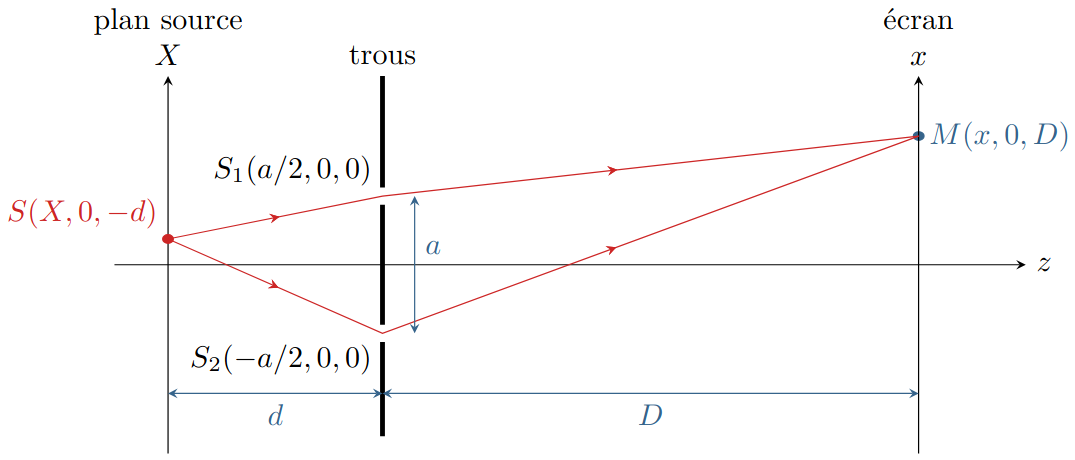
\includegraphics[width=0.9\linewidth]{source_decalee.png}
	\caption{Schéma de l'expérience des trous d'Young, avec une source décalée selon $(Ox)$.}
\end{figure}

Expérimentalement, si on réalise l'expérience, on constate que l'on a toujours des franges avec le même interfrange $i$, mais elles sont décalées.

\begin{capex}
	Montrer ce résultat et déterminer la position de l'ordre d'interférences $p=0$ en fonction de $X$. Déterminer l'ordre d'interférences en $x=0$.
\end{capex}

\subsubsection{Critère de brouillage pour une source étendue}

On considère désormais une source étendue de largeur $b$ entre les positions $X = -b/2$ et $X = +b/2$.

\begin{capex}
	A partir du critère de brouillage des interférences, déterminer à partir de quelle largeur $b$ de la source les interférences sont brouillées.
\end{capex}

On en déduit la condition suivante de brouillage des interférences sur la largeur angulaire de la source :
\begin{proposition}[Critère de perte de cohérence spatiale]
	Dans le cas d'une source étendue, on va avoir brouillage des interférences lorsque l'angle $\theta_S \approx \frac{b}{d}$ sous lequel est vu la source depuis les trous d'Young dépasse une valeur critique :
	\begin{equation}
		\theta_{S,lim} = \frac{\lambda}{a}
	\end{equation}
	Le brouillage est uniforme sur l'écran, et on dit alors que l'on a perte de cohérence spatiale.
\end{proposition}
\begin{remark}
	On peut remarquer que cet angle limite correspond à l'angle auquel la lumière serait diffractée par les trous d'Young si elle se propageait en sens inverse. De plus, on remarque aussi que le brouillage est uniforme, ce qui n'était pas le cas lorsqu'on a perte de cohérence temporelle.
\end{remark}

\subsubsection{Pour aller plus loin : calcul exact du facteur de contraste}

\textit{Les propriétés et démonstrations présents dans cette partie ne sont pas exigibles.}

Il est possible de s'affranchir du critère de brouillage en calculant directement l'intensité lumineuse sur l'écran pour une source étendue, et de déterminer son contraste.
\begin{proposition}[Contraste des franges en fonction de la largeur de la source]
On peut montrer que l'intensité sur l'écran s'écrit :
\begin{equation}
	I_{tot} = I_0 \left( 1 + C(b) \cos\left(2 \pi \frac{\delta}{\lambda} \right) \right)
\end{equation}
où le facteur de contraste est fonction de la largeur $b$ de la source :
\begin{equation}
	C(b) = \mathrm{sinc}\left( \frac{\pi a b}{\lambda d}  \right)
\end{equation}
\end{proposition}

\begin{demonstration}
Pour obtenir cette expression, on découpe la source étendue, émettant une intensité $I_0$ en une somme de sources de largeur $\dd X$ et d'intensité $\dd I = I_0 \frac{\dd X}{b}$. Alors comme ces sources sont toutes incohérentes, les figures d'interférences associées s'ajoutent :
\begin{align}
	I_{tot} &= \int_{-b/2}^{b/2} I_0 \frac{\dd X}{b} \left[ 1 + \cos( 2 \pi p_{x}(M))\right] \quad \mathrm{avec} \quad p_X(M) = \frac{aX}{\lambda d} + \frac{ax}{\lambda D}
	&= I_0 + \frac{\lambda d}{2 \pi a b} \left[ \sin\left(\frac{2 \pi a}{\lambda} \left(\frac{X}{d} + \frac{x}{D}\right) \right) \right]_{-b/2}^{b/2}
\end{align}
On peut alors utiliser la formule :
\begin{equation}
	\sin p - \sin q = 2 \sin \frac{p-q}{2} \cos \frac{p+q}{2}
\end{equation}
pour remarquer que :
\begin{equation}
	\left[ \sin\left(\frac{2 \pi a}{\lambda} \left(\frac{X}{d} + \frac{x}{D}\right) \right) \right]_{-b/2}^{b/2} = 2 \sin\left(\frac{\pi a b}{\lambda d}\right) \cos\left( \frac{2 \pi}{\lambda} \frac{a x}{D} \right)
\end{equation}
	On obtient alors directement le résultat à prouver, en reconnaissant la différence de marche $\delta = \frac{a}{x}{D}$.
\end{demonstration}



\begin{figure}[htbp]
	\centering 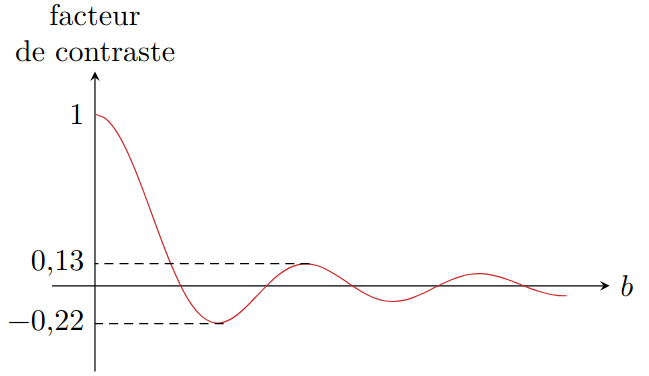
\includegraphics[width=0.5\linewidth]{contraste_sinc.png}
	\caption{Facteur de contraste en fonction de la largeur de la fente source.}
\end{figure}

On constate clairement que le facteur de contraste est une fonction progressive : il n'est pas égal à 1 en dessous du critère de brouillage et à 0 au-dessus de ce critère. Il diminue prograssivement (en valeur absolue), au fur et à mesure que l'on augmente la largeur de la fente. On observe des annulations de contraste (brouillage total des interférences) pour certains valeurs bien particulières de la largeur $b$ de la source lumineuse.


\section{Réseaux}




\end{document}
